\RequirePackage[]{lineno}
\documentclass[12pt]{article}
\usepackage{caption}
\usepackage{times}
\usepackage{setspace}
\usepackage{longtable}
\usepackage{amsmath}
\usepackage{booktabs}
\usepackage{float}
\usepackage{mathpazo}
\usepackage{times}
\usepackage{tikz}
\usepackage{graphicx}
\usepackage[hmargin=2.25cm, vmargin=2cm, headheight=15.5pt]{geometry}
\usepackage{multirow}
\usepackage{tcolorbox}
\usepackage{multicol}
\usepackage{tabularx}
\usepackage{rotating}
\usepackage{pdflscape}


\captionsetup[figure]{font=small}
\captionsetup[table]{font=small}

\usetikzlibrary{arrows,calc}
\geometry{margin=1in}

%\captionsetup{font=doublespacing, size= footnotesize}% Double-spaced float captions
\doublespacing
\DeclareCaptionJustification{double}{\DoubleSpacing}
% Reasonable page setup


\usepackage[]{natbib}
\bibpunct[; ]{(}{)}{;}{a}{,}{;}

% to avoid things being lost to overleaf comment bubbles
\long\def\authornote#1{%
    \leavevmode\unskip\raisebox{-3.5pt}{\rlap{$\scriptstyle\dagger$}}%
    \marginpar{\raggedright\hbadness=10000
        \def\baselinestretch{0.8}\tiny
        \it #1\par}}
\newcommand{\DBS}[1]{\authornote{DBS: #1}}
\newcommand{\ACL}[1]{\authornote{ACL: #1}}

\usepackage{authblk}
\renewcommand\Affilfont{\small}

\newenvironment{abox}[1]{
  \begin{tcolorbox}[float,title=#1, colback=blue!4]
  \fontsize{9}{10}\selectfont
  \begin{multicols}{2}
}{
  \end{multicols}
  \end{tcolorbox}
}


\newenvironment{ecolettcover}{\maketitle}{\clearpage}
\newenvironment{ecolettabstract}{\clearpage\section*{Abstract}}{\clearpage}
\tikzset{
	%Define standard arrow tip
	>=stealth',
	%Define style for different line styles
	help lines/.style={dashed, thick},
	axis/.style={<->},
	important line/.style={thick},
	connection/.style={thick, dotted},
}

%\title{The structural sensitivity of competition models: how model formulation changes our predictions of species coexistence}
\title{Quantifying the relative contribution of environmental fluctuations to the maintenance of a sexually antagonistic polymorphism}
\author[1]{Alba Cervantes-Loreto}
\author[1]{Michelle L.\ Marraffini}
\author[1]{Daniel B.\ Stouffer}
\author[1]{Sarah P.\ Flanagan}


\affil[1]{Centre for Integrative Ecology, School of Biological Sciences\\ University of Canterbury, Christchurch 8140, New Zealand}



% Include the date command, but leave its argument blank.
\date{}

%%%%%%%%%%%%%%%%% END OF PREAMBLE %%%%%%%%%%%%%%%%
\let\oldequation\equation
\let\oldendequation\endequation

\renewenvironment{equation}
  {\linenomathNonumbers\oldequation}
  {\oldendequation\endlinenomath}

% \pagestyle{empty}

\begin{document}
\linenumbers
% Double-space the manuscript.
\baselineskip30pt
\maketitle

\begin{ecolettcover}

%\centerline{{\sc Running Title:} The structural sensitivity of competition models}
\begin{center}
\begin{tabular}{ll}
\hline \\

\bf{Words in abstract}         & 203 \\
\bf{Words in manuscript}       & 5130\\
\bf{Number of references}      & 50  \\
\bf{Number of figures}			& 4 \\
\bf{Number of tables} 			& 2 \\
\bf{Number of text boxes}		& 0 \\
\bf{Corresponding author}      & Alba Cervantes-Loreto \\
\bf{Phone}                     & +64~369~2880 \\

\bf{Email}                     & alba.cervantesloreto@pg.canterbury.ac.nz \\
                                                                        \\
\hline
\end{tabular}
\end{center}

\maketitle

\end{ecolettcover}
\section{Abstract}



Sexually antagonistic selection (SAS) occurs when the selection in the traits or loci differs between the sexes. This sexual conflict offers the opportunity for maintaining polymorphism in a population, but it often results in the eventual fixation of the fitter allele. However, the effects of SAS have generally been studied under strong simplifying assumptions, such as constant populations and homogeneous environments, which could considerably change the expected outcomes of SAS. Thus, in this study, we examined how fluctuations in selection and population sizes contributed to the coexistence of sexually antagonistic alleles by adopting an ecological framework that allowed us to examine evolutionary dynamics through the same lens as the coexistence of competing species. We performed simulations of alleles invading a population while allowing selection and populations sizes to fluctuate over time.  Then, we quantified coexistence outcomes and the relative contribution of each type of fluctuation to each alleles' invasion growth rate. Our results showed that environmental fluctuations can dramatically increase the expected genetic variation under SAS. The positive contribution of fluctuations, however, depended on the sex and allele where invasion occurred. This study contributes to the growing body of work that shows the importance of non-constant environments on the maintenance of genetic diversity.

\section{Introduction}
The question of how genetic variation is maintained despite the effects of selection and drift is central within evolutionary biology \citep{walsh_evolution_2018}. Classical explanations include overdominance (heterozygote advantage) or frequency-dependent selection \citep{hedrick2007balancing}, but in the modern era of genomic data, all patterns of variation that exceed the expected variation under neutrality tend to be categorized broadly as balancing selection, regardless of the evolutionary mechanism \citep{mitchell-olds_which_2007}. In species with separate sexes, balancing selection can arise due to sexually antagonistic selection \citep{connallon2014balancing}, which occurs when the direction of natural selection on traits or loci differs between the sexes \citep{lande1980sexual,arnqvist2013sexual}.


Sexually antagonistic selection can maintain polymorphisms of otherwise disadvantageous alleles in a population \citep{gavrilets2014sexual}, which in turn can result in phenotypically distinct sexes that express different morphological, physiological, and behavioral traits \citep{mori2017sexual,connallon2018environmental}. Nonetheless,
the extent to which sexually antagonistic selection can maintain polymorphism in a population is thought to be limited \citep{connallon2012general,connallon2018environmental}. This is because theoretical studies have found that the necessary parameter conditions that give rise to balancing selection are often highly restrictive \citep{kidwell1977regions,pamilo1979genic,hedrick1999antagonistic,curtsinger1994antagonistic, patten2010fitness, jordan2012potential}. Importantly, the effect of sexually antagonistic selection generally has been studied under strong simplifying assumptions such as constant population sizes and homogeneous environments  \citep{kidwell1977regions, pamilo1979genic, immler2012ploidally, jordan2012potential}. Studies that have explored the effect of sexually antagonistic selection with more realistic assumptions, such as temporal fluctuations in selection \citep{connallon_evolutionary_2018} or demographic fluctuations \citep{connallon2012general} have found that polymorphism can be maintained in a much wider set of conditions than classical studies predict. These results suggest that environmental fluctuations are essential to fully understand the effects of sexually antagonistic selection.

The contribution of environmental fluctuations to genetic diversity remains a debated issue in evolutionary biology. Classic theoretical models predict that temporal fluctuations in environmental conditions are unlikely to maintain a genetic polymorphism in haploid populations \citep{dempster1955maintenance,hedrick1974genetic,hedrick1986genetic}. However, other studies have found that fluctuating selection can maintain genetic variance when populations experience density dependence \citep{dean2005protecting}, on sex-linked traits \citep{reinhold2000maintenance}, or in populations where generations overlap \citep{ellner1994role, ellner1996patterns}. Similarly, temporal changes in population sizes have been shown to mitigate the effect of genetic drift in small populations \citep{pemberton1996maintenance} and in annual plant systems \citep{nunney2002effective}. Importantly, progress requires more than just identifying if environmental fluctuations can maintain genetic diversity in a population, but to quantify how exactly they contribute to its maintenance \citep{ellner2016quantify}.

The mechanisms by which environmental fluctuations promote diversity maintenance have been thoroughly  studied in ecological contexts \citep{levins1979coexistence,armstrong1980competitive,chesson2000general,barabas_chessons_2018}. Note that from an ecological perspective, polymorphism of sexually antagonistic alleles is equivalent to the coexistence of species, and the fixation of either one of the alleles in a population is equivalent to competitive exclusion. Allelic polymorphism, thus, can be examined through the same lens as the coexistence of competing species. \citep{ellner1994role,ellner1996patterns,dean2005protecting,schreiber2010interactive}. The benefit of analyzing evolutionary dynamics through this lens is that the main theoretical framework used to examine how competing species coexist, often called Modern Coexistence Theory \citep{Chesson2000, barabas_chessons_2018}, allows the quantification of how environmental fluctuations contribute to coexistence. Despite that the use of Modern Coexistence Theory often requires complex mathematical analysis of the models describing the systems dynamics and restrictive assumptions \citep{barabas_chessons_2018}, recent computation approaches allow the quantification of the relative importance of environmental fluctuations to coexistence using simulations \citep{ellner2016quantify,ellner_expanded_2019,shoemaker2020}.

Here, we seeked to explicitly quantify how temporal environmental fluctuations contribute to the maintenance of polymorphism under sexually antagonistic selection by applying recent advances in Modern Coexistence Theory.  We examined how fluctuations in selection values, fluctuations in population sizes, and their interactions can further or hinder polymorphism. In particular, we examined i) Can fluctuations in population sizes and selection values allow sexually antagonistic alleles to coexist when differences in their fitness would typically not allow them to? and ii) What are the relative contributions of different types of fluctuations that allow two sexually antagonistic alleles to be maintained in a population? Our study provides the tools to analyze sexual antagonism from a novel perspective and contributes to answering long-lasting questions regarding the effect of non-constant environments on genetic diversity.


\section{Methods}

We first present a model that describes the evolutionary dynamics of sexually antagonistic alleles. We then show how we simulated different scenarios of alleles invading a population, where we allowed population sizes, selection, both, or neither to vary. Finally, we detail how we examined the relative contribution of each type of fluctuation to the maintenance or loss of polymorphism.

\subsection*{Population dynamics of sexually antagonistic alleles}


Our model examined evolution at a single, biallelic locus. We further assumed the relative fitness of each allele was frequency and density independent. We examined the dynammics of two  sexually antagonistic alleles, $j$ and $k$, that affect fitness in the haploid state. The frequencies of each allele in each sex at the beginning of a life-cycle at generation $t$ are given by:
\begin{equation}
    p_{jm,t}= \frac{n_{jm,t}}{N_{m,t}}
    \label{first_pop}
\end{equation}
\begin{equation}
    p_{jf,t}= \frac{n_{jf,t}}{N_{f,t}}
\end{equation}
\begin{equation}
    p_{km,t}=  \frac{N_{m,t}-n_{jm,t}}{N_{m,t}}
\end{equation}
\begin{equation}
    p_{kf,t}= \frac{N_{f,t}-n_{jf,t}}{N_{f,t}}
\end{equation}
where $N_{m,t}$ and $N_{f,t}$ are the total numbers of males and females in the population at generation $t$, $n_{jf,t}$ is the number of females $f$ with allele $j$, and $n_{jm,t}$ is the number of males $m$ with allele $j$ at time $t$, respectively. Consequently, the number of males with allele $k$ at generation $t$ is given by $n_{km,t}=N_{m,t}-n_{jm,t}$ and the number of females by $n_{kf,t}=N_{f,t}-n_{jf,t}$.

The individuals in the population mate at random before selection occurs, and therefore the frequency of offspring with allele $j$ after mating, $p'_{j,t}$ can be expressed as:
\begin{equation}
   p'_{j,t}= \frac{n_{jf}}{N_{f}} \frac{n_{jm}}{N_{m}} + \frac{1}{2} \frac{n_{jf}}{N_{f}} \frac{(N_{m}-n_{jm})}{N_{m}} +\frac{1}{2}
   \frac{(N_{f}-n_{jf})}{N_{f}} \frac{n_jm}{N_{m}}
   \label{prime_a}
\end{equation}
which upon rearranging and simplifying gives:
\begin{equation}
   p'_{j,t}= \frac{N_{m,t}n_{jf,t}+ N_{f,t}n_{jm,t}}{2 N_{f}N_{m}}
   \label{pprime}
\end{equation}

For simplicity, we use allele $j$ as an example. However, an equivalent expression for allele $k$ can be obtained by interchanging $k$ subscripts for $j$ in Eqn.~\ref{prime_a}. Selection acts upon these offspring in order to determine the allelic frequencies in females and males in the next generation, $t+1$. As an example, the frequency  of females with allele $j$ after selection is given by:
\begin{equation}
   p_{jf, t+1}= \frac{n_{jf, t+1}}{N_{f,t+1}} = \frac{p'_{j,t}w_{jf}}{p'_{t,j}w_{jf}+ (1-p'_{t,j})w_{kf}}
   \label{next_gen}
\end{equation}

The logarithmic per capita growth rate of allele $j$ in females is therefore given by the number of females carrying allele $j$ after selection divided by the original number of females carrying allele $j$:

\begin{equation}
    r_{jf,t} = \ln \left( \frac{n_{jf, t+1}}{n_{jf,t}} \right)
    \label{canonical}
\end{equation}

An equivalent expression for the logarithmic per capita growth rate of allele $j$ in males $m$ can be obtained by exchanging $f$ for $m$ across the various subscripts in Eqn.~\ref{next_gen}.

Polymorphism in a sexual population, however, is ultimately influenced by growth and establishment of an allele across both sexes. Therefore, the growth rate of allele $j$ across the entire population of females \emph{and} males is given by:
\begin{equation}
    r_{j,t} = \ln \left( \frac{n_{jf, t+1} + n_{jm, t+1} }{n_{jf,t} + n_{jf,t} }  \right)
    \label{full}
\end{equation}
An equivalent expression describes $r_{k,t}$, the growth rate of allele $k$.


Our model further assumed allele $j$ always has a high fitness in females ($w_{jf} = 1$) but variable fitness in males ($w_{jm} < 1$); and allele $k$ has a high fitness in males ($w_{km} = 1$)  but variable fitness in females ($w_{kf} < 1 $). The selection against allele $j$ in males is therefore $S_{m}= 1 - w_{jm}$, and the selection against allele $k$ in females is $S_{f}= 1 - w_{kf}$. When population sizes and selection values are constant,
selection mantains both alleles in the population, under the condition that:

\begin{equation}
\frac{S_{m}}{1+S_{m}} < S_{f} < \frac{S_{m}}{1-S_{m}}
\label{selection}
\end{equation}
\citep{kidwell1977regions,pamilo1979genic,patten2010fitness,connallon_evolutionary_2018}. Thus, the maintenance of polymorphism of sexually antagonistic alleles is solely determined by the values of $S_{m}$ and $S_{f}$. Note that in our model, the values $S_{m}$ and $S_{f}$ are bounded from $0$ to $1$. Therefore the parameter space of sexually antagonistic selection is within the range $ 0< S_{m}, S_{f} < 1$. Classic theoretical models predict that, in constant environments, polymorphism is maintained in $\approx 0.38$ of the parameter space \citep{kidwell1977regions,pamilo1979genic,connallon_evolutionary_2018}. Nonetheless, it is unrealistic to assume population sizes and selection are constant through time. Temporal changes in population densities are ubiquitous in nature \citep{connallon2012general,reinhold2000maintenance}. Similarly, the effect of sexual selection has been shown to vary through space and time \citep{kasumovic2008spatial}. If fluctuations in population sizes or selection values affect the coexistence of sexually antagonistic alleles, it would be reflected in increases or decreases of the proportion of the parameter space where polymorphism is maintained.

\subsection*{Simulations}
We examined the effect of fluctuating population sizes and selection in the maintenance of a genetic polymorphism across the parameter space ($0 < S_{m}, S_{f} < 1$). To do so, we partitioned the parameter space into a $50 \times 50$ element grid, which yielded 2500 pairwise combinations of different $w_{jm}$ and $w_{kf}$ values. For each pairwise combination of $w_{jm}$ and $w_{kf}$, as we detail in the next sections, our simulation approach consisted of three main parts. First, we incorporated fluctuations in population sizes and selection into our population dynamics model. Second, we performed simulations to evaluate if both alleles could establish when the environment fluctuated. Finally, we determined the relative contribution of each type of fluctuation to the establishment of each allele.

For each grid we controlled the effect size of  fluctuations in selection ($\sigma_{w}$) and their correlation ($\rho_{w}$), as well as fluctuations in population sizes ($\sigma_{g}$) and their correlation ($\rho_{g}$). We explored all of  the combinations of low ($\sigma_{w}\in{(0.1, 0.3)}$, $\sigma_{g}\in{(1,10)}$), intermediate ($\sigma_{w}\in{(0.5, 0.7)}$, $\sigma_{g}\in{(20,30,50)}$), and high fluctuations ($\sigma_{w}= 0.9$, $\sigma_{g}=70$)  in selection values and population sizes, with different extents of correlations between fluctuations (Table \ref{tab:fluctuations}).  As a control simulation, we set $\sigma_{w}= 0$ and  $\sigma_{g}=0$, with no correlation between fluctuations. We ran ten replicates per parameter combination, which resulted in 3780 grids.
\subsubsection*{Timeseries}

To incorporate the effects of fluctuations into our population dynamics model we generated independent timeseries of fluctuations in selection and population sizes. In the case of fluctuations in selection values, for a given value of $w_{jm}$ and $w_{kf}$ (i.e., a fixed point in the selection parameter space), we generated a timeseries of 500 generations made up of correlated fluctuations of $w_{jm}$ and $w_{kf}$. We controlled the size of  fluctuations in selection ($\sigma_{w}$) and correlation between sexes ($\rho_{w}$) by  using the variance-covariance matrix:

\begin{equation}
C_{w} = \begin{bmatrix}
\sigma_{w}^{2} & \rho_{w} \sigma_{w}^{2} \\
\rho_{w} \sigma_{w}^{2} & \sigma_{w}^{2}
\end{bmatrix}
\label{covmat}
\end{equation}

We then, performed a Cholesky decomposition of Eqn.~\ref{covmat} and multiplied it by a ($2 \times 500$) matrix of random numbers from a normal distribution, which yielded $\gamma_{j,t}$ and $\gamma_{k,t}$. Since fitness values are bounded from zero to one, we added fluctuations in a logistic space. Therefore, we transformed fitness values as $w'_{jm} = \ln\frac{w_{jm}}{1-w_{jm}}$ and $w'_{kf} = \ln\frac{w_{kf}}{1-w_{kf}}$. Finally, we calculated the fitness values at generation $t$ as:

\begin{eqnarray}
  w_{jm,t}= \frac{e^{-(w'_{jm}+ \gamma_{j,t})}}{(1+ e^{-(w'_{jm}+ \gamma_{j,t})})^2} \\
    w_{kf,t}= \frac{e^{-(w'_{kf}+ \gamma_{k,t})}}{(1+ e^{-(w'_{kf}+ \gamma_{k,t})})^2}
\end{eqnarray}

This approach guaranteed that fluctuations in $w_{jm}$ and $w_{kf}$ were always bounded from zero to one.

Similarly, we generated an independent timeseries of 500 generations made up of correlated fluctuations in population sizes.  We again used a Cholesky factorization of the variance-covariance matrix, to control the size of fluctuations in population sizes with $\sigma_{g}$ and their correlation with $\rho_{g}$. Similar to our previous approach, we multiplied this factorization by a random matrix of uncorrelated unit normal random variables, which yielded $\gamma_{m,t}$ and $\gamma_{f,t}$. Finally, we calculated the number of males and females in the population at generation $t$ as $N_{m,t} = N_{m,0} + \gamma_{m,t}$ and $N_{f,t} = N_{f,0}+ \gamma_{f,t} $. Therefore, the population sizes in each generation differed from the initial value on the order of $\sigma_{g}$. To avoid extinction due to fluctuations in population sizes, we imposed a lower bound on the population sizes of both sexes of one individual. Note that the scales of $\sigma_{g}$ and  $\sigma_{w}$ are different from each other. While $\sigma_{w}$ controls the change in fitness values in logistic space, $\sigma_{g}$ controls the number of individuals added or removed to a population.

%We bounded the values population sizes could take so there were no negative population sizes since that would not be biologically plausible. We did not impose an upper bound to the values population sizes could take.

%We chose values of $N_{m}= 200$ and $N_{f}=200$ as the initial value of population sizes throughout our simulations.

Finally, we performed simulations where our population dynamics model (Eqns.~\ref{first_pop} to \ref{full}) was iterated over 500 generations while allowing selection values and population sizes to fluctuate in each generation. We started each simulation with the initial values of $N_{m,0}=200$ and $N_{f,0}=200$ and equal frequencies of allele $j$ and allele $k$ in each sex. For each generation $t$ in our simulations, the values of $w_{jm,t}$ $w_{kf,t}$, $N_{m,t}$ and $N_{f,t}$ used to calculate allele's frequencies in generation $t$ (e.g., Eqn.~\ref{next_gen}), corresponded to the $t$ values calculated in each timeseries, as described previously. This approach yielded a final timeseries that captured the dynamics of sexually antagonistic alleles with fluctuating values of selection and population sizes.

\subsubsection*{Invasion simulations}

 To evaluate if both alleles could establish when the environment fluctuated, we turned towards criteria from Modern Coexistence Theory criteria to evaluate coexistence. Modern Coexistence Theory has shown that coexistence is promoted by mechanisms that give species a population growth rate advantage over other species when they become rare \citep{chesson_stabilizing_1982, chesson2003quantifying, barabas_chessons_2018}. Typically, one species is held at its \textit{resident} state, as given by its steady-state abundance while the rare species is called the \textit{invader}. In the context of alleles in a population, an allele is an \textit{invader} when a mutation occurs that introduces that allele into a population in which it is absent (e.g., in a population with only $k$ alleles, if a random mutation leads to one individual carrying the $j$ allele). Within sexually antagonistic selection, each allele has two pathways of invasion, depending on whether the mutation arises in a female or in a male. If an allele's \textit{invasion growth rate} (or the average instantaneous population growth rate when rare) is positive, it buffers it against extinction, maintaining its persistence in the population.  Coexistence, and hence polymorphism, occurs when both alleles have positive invasion growth rates.

We used the timeseries that captured the dynamics of our population model with environmental fluctuations as a template to perform invasion simulations of both alleles. Following the approach of \citet{shoemaker2020}, we treated each invasion simulation independently, and hence we performed 500 invasion simulations, one for each generation in our timeseries. We explored all four potential combinations of each allele invading through each pathway (e.g., allele $j$ invading through males, allele $k$ invading through females, and so on). To simulate invasion, we set the density of the invading allele to one individual. Since we treated each invasion simulation as independent, we denoted the initial timestep in an invasion simulation with the subscript $i$. For example, if allele $j$ was invading via males, then we would set $n_{jm,i} = 1$ and $n_{jf,i}= 0$. We also set the resident allele, in this case $k$, to the corresponding value of the timeseries minus one individual, $n_{km,i} = N_{m,t} -1$ and $n_{kf,i} = N_{f,t}$. We then simulated invasion by iterating our population dynamics model one generation, $i+1$, and calculated the logarithmic growth rate of the invading allele, which in this case would be given by:
 %We allowed each allele to invade via two different pathways: males and females
%For each timestep in the timeseries, we performed simulations of the two alleles invading separately via their respective pathway.


\begin{equation}
r_{j,i} =	\ln \left ( \frac{n_{jm,i+1 } + n_{jf,i+1}}{1} \right )
\label{invader}
\end{equation}

Similarly, the logarithmic growth rate of the resident allele would be given by:
\begin{equation}
r_{k,i} =	\ln \left ( \frac{ n_{km,i+1} + n_{kf,i+1} }{ n_{km,i} + n_{kf,i}  } \right )
\label{resident}
\end{equation}

We performed invasion simulations for each allele invading via  each potential pathway. We then calculated the mean invasion growth rate of each allele as an invader as the average of the 500 invasion growth rates. We also calculated the mean growth rate of each allele as a resident as the average of the 500 resident growth rates. We determined alleles could coexist  and therefore polymorphism to be maintained in a point in the parameter space if both of alleles had positive mean invasion growth rates, which is often referred to as the mutual invasibility criterion \citep{barabas_chessons_2018}.


\subsubsection*{Functional decomposition}


Our invasion simulations evaluated whether or not polymorphism can be maintained in a determined point of the selection parameter space when the environment fluctuates. However, we also quantified the relative contributions of fluctuations in selection and population sizes to the predicted coexistence outcome using a \textit{functional decomposition} approach \citep{ellner2016quantify,ellner_expanded_2019, shoemaker2020}.

%also wanted to quantify the relative contributions of fluctuating selection and population sizes into the predicted coexistence outcome. Therefore, we turned towards an extension of modern coexistence theory \citep{ellner_expanded_2019} that provides the flexibility to analyze the contributions of different processes to coexistence using \textit{functional decomposition}. This approach applies to any collection of two or more processes, mechanisms, or species differences affecting population growth rate \citep{ ellner2016quantify, ellner_expanded_2019}, and has been used to show the relative contribution of variable temperature and silicate to the coexistence of algal species \citep{ellner2016quantify} and to quantify the relative importance of environmental fluctuations and variation in predator abundances to the coexistence of intertidal species \citep{shoemaker2020}.


%Modern coexistence theory provides an analytical framework to decompose each allele´s, invasion growth rates into a sum of terms for the effects of different factors, such as abiotic and biotic fluctuations, and then compare invader and residents term by term \citep{ellner_expanded_2019}. Mechanisms that promote coexistence can help whichever allele is rare, or it can hurt whichever allele is common. Therefore, to understand the role of each mechanism, it is necessary to compare how it affects invader \textit{and} resident growth rates.

%modern coexistence theory uses Taylor series expansion to do this decomposition and comparison (a detailed review can be found in \citet{barabas_chessons_2018}). We present an analytical approach, using classic modern coexistence theory, to understand the relative contributions of fluctuation in population sizes and fitness values to each alleles' growth rate as an invader in the Supporting Information.

The functional decomposition approach separates the average growth rate of each allele into a null growth rate in the absences of fluctuations in all selected variables, a set of main effect terms that represent the effect of only one variable fluctuating, a set of two-way interaction terms representing the effect of variables fluctuating simultaneously, and so on \citep{ellner_expanded_2019}. In our simulations, this is a function of four variables: the number of males in the population ($N_{m}$), the number of females in the population ($N_{f}$), the fitness of allele $j$ in males ($w_{jm}$), and the fitness of allele $k$ in females ($w_{kf}$). As a simplified example, if only $N_{m}$ and $N_{f}$ were fluctuating, the growth rate of allele $j$ when it is the invader (Eqn.~\ref{invader}) at invasion time $i$ could be decomposed into:

\begin{equation}
   r_{j,i}(N_{m},N_{f}) = \mathcal{E}_{j}^{0} + \mathcal{E}_{j}^{N_{m}}+ \mathcal{E}_{j}^{N_{f}}+ \mathcal{E}_{j}^{N_{m}N_{f}}
   \label{functional_decomp}
\end{equation}
Where $\mathcal{E}^0$ is the null growth rate when $N_{m}$ and $N_{f}$ are set to their averages. Terms with superscripts represent the marginal effects of letting all superscripted variables vary while fixing all the other variables to their average values. For example, the term $\mathcal{E}_{j}^{N_{m}}$ expresses the contribution of fluctuations in $N_{m}$ when $N_{f}$ is set to its average, without the contribution when both variables are set to their averages :

\begin{equation}
  \mathcal{E}_{j}^{N_{m}} = r_{j,i}(N_{m},\overline{N_{f}}) - \mathcal{E}_{j}^{0}
\end{equation}

If we average Eqn.~\ref{functional_decomp} across generations, we get a partition of the average population growth rate into the variation free growth rate, the main effects of variability in $N_{m}$, the main effects of variability in $N_{f}$, and the interaction between variability in $N_{m}$ and $N_{f}$:

\begin{equation}
    \overline{r}_{j}= \mathcal{E}_{j}^{0} + \overline{\mathcal{E}_{j}}^{N_{m}}+ \overline{\mathcal{E}_{j}}^{N_{f}}+ \overline{\mathcal{E}_{j}}^{N_{m}N_{f}}
   \label{functional_decomp_2}
\end{equation}

In our simulations $w_{jm}$ and $w_{kf}$ also fluctuated, therefore the full functional decomposition of the growth rate of allele $j$ as an invader is found in Table \ref{tab:EllnerRs}, as well as a brief description of the meaning of each term. For simplicity we only show terms related to allele $j$ as an invader, however, the functional decomposition approach can be applied analogously when allele $k$ invades. Note that Table \ref{tab:EllnerRs} does not include three or four-way interactions (e.g., $\overline{\mathcal{E}_{j}}^{N_{m}N_{f}w_{jm}w_{fk}}$). This is because in our simulations, we did not allow fluctuations in selection and population sizes to be correlated, therefore their effects are solely captured by the terms in Table \ref{tab:EllnerRs}. We calculated the value of each of the terms in Table \ref{tab:EllnerRs} by performing another set of invasion simulations controlling which variables were allowed to fluctuate. For example, to calculate the value of $\mathcal{E}_{j}^{0}$ we performed another 500 simulations of allele $j$ invading but instead of using the values of $w_{jm,i}$ $w_{kf,i}$, $N_{m,i}$ and $N_{f,i}$ used to calculate the frequency of allele $j$ in generation $i+1$, we set the all the variables to their mean values. Then, to calculate the value of $\mathcal{E}_{j}^{N_{m}}$, we set all variables except  $N_{m}$ to their mean values and subtracted the value of $\mathcal{E}_{j}^{0}$, and so on with subsequent terms.

The functional decomposition approach further allows the \textit{comparison} of each term to understand if how it affects invaders and residents (i.e., the relative contribution). This is because fluctuations can promote the maintenance of polymorphism by helping whichever allele is rare, or by hurting whichever allele is common. Therefore, to understand the role of each type of fluctuation, it is necessary to compare how it affects both invader \textit{and} resident growth rates. In the example presented in Eqn.~\ref{functional_decomp_2}, if allele $j$ is invading, then allele $k$ is at it's resident state and there exists an analogous decomposition of $\overline{r}_{k}$. Therefore we can express the difference between contributions of fluctuations in $N_{m}$ as:


\begin{equation}
\Delta^{N_{m}}_{j}= \overline{\mathcal{E}_{j}}^{N_{m}} - \overline{\mathcal{E}_{k}}^{N_{m}}
\label{delta}
\end{equation}

If $\Delta^{N_{m}}_{j}$ is positive, then fluctuations in the male population size benefit allele $j$ when it is rare more than they benefit $k$ as a resident. If $\Delta^{N_{m}}_{j}$ is negative, then fluctuations benefit $k$ as a resident more than $j$ as an invader. Therefore, for each allele invading via a different pathway, we calculated 7 separate $\Delta$ values, one for each one of the $\mathcal{E}$ terms in Table \ref{tab:EllnerRs}.


In the course of our analysis we noticed that the magnitude of each one of the $\Delta$ values could vary considerably across the parameter space. To make them comparable and ease interpretation, we normalized each $\Delta$ value by dividing it by the square root of the sum of the squares of the 7 $\Delta$ values. For example, the normalized value of Eqn.~\ref{delta} would be given by:



\begin{equation}
  \delta^{N_{m}}_{j}= \frac{\Delta^{N_{m}}_{j}}{\sqrt{
    \sum\limits_{d=1}^{7} (\boldsymbol{\Delta_{d}})^{2} }}
\end{equation}

This normalization bounded $\delta$ values from $-1$ to $1$. Similar to the interpretation of $\Delta$ terms, positive $\delta$ values mean that fluctuations benefit an allele as an invader more than the other allele as a resident and negative $\delta$ values imply that fluctuations do not benefit an allele as an invader more than the other allele as a resident.


\section{Results}
Our results showed that both fluctuations in selection and population sizes can substantially increase the expected genetic variability under sexually antagonistic selection. The proportion of the parameter space where polymorphism was maintained increased with the effect size of both types of fluctuations (Fig.~\ref{fig:heatmap}). Increases in the proportion of polymorphism were more likely when fluctuations in selection and population sizes were large, fluctuations in population sizes were negatively correlated, and fluctuations in selection were positively correlated. Importantly, our results show that environmental fluctuations can increase the proportion of allelic polymorphism up to $0.6$ (Fig.~\ref{fig:heatmap}).

Our results matched previous findings that without fluctuations, polymorphism can be maintained in only $ 0.38$ of the parameter space (Fig.~\ref{fig:outcomes}A). Increments in polymorphism when population sizes fluctuated occurred near the limit of the domain of balancing selection and were particularly pronounced when selection against both alleles was weak (Fig.~\ref{fig:outcomes}B). When selection against either of the alleles was strong ($ S_{m}, S_{f}> 0.75 $), fluctuations in population sizes did not increase polymorphism compared to the control (Fig.~\ref{fig:outcomes}B). Similarly, increments in polymorphism when selection fluctuated also occurred near the limit of the domain of balancing selection, however, fluctuations in selection did not affect polymorphism when selection against both alleles was weak ($ S_{m}, S_{f}< 0.25 $) (Fig.~\ref{fig:outcomes}C). When both population sizes and selection fluctuated, increments in polymorphism occurred near the limit of the domain of balancing selection, regardless of the strength of selection

The effect of fluctuations in population sizes and selection was not homogeneous across the parameter space. The values of $\delta^{0}$ followed the effect of selection outlined by Eqn.~\ref{selection} (Fig.~\ref{fig:space}). Note that near the limit of the domain of selection, the effect of $\delta^{0}$ was close to zero. In contrast, the rest of the $\delta$ values were generally stronger in magnitude near the limit of the domain of selection  (Fig.~\ref{fig:space}). Despite their similar patterns in the parameter space, the role of each type of fluctuation to the growth rate of alleles when rare depended on the allele and pathway where the invasion took place(Fig.~\ref{fig:space}).

Fluctuations in population sizes of males and females benefited alleles when alleles invaded via the fluctuating population (Fig.~\ref{fig:boxes}). In contrast, fluctuations in the population of one sex made it more difficult for either allele to invade via the other sex (Fig.~\ref{fig:boxes}). For example, the relative contribution of fluctuations in the male population, $\delta^{N_{m}}$, was positive for both alleles when they invaded via males and negative when they invaded via females, regardless of the correlation between fluctuations (Fig.~\ref{fig:boxes}). The relative contribution of both populations fluctuating,  $\delta^{N_{m}N_{f}}$, was positive when fluctuations were negatively correlated, had a negligible effect when fluctuations were not correlated, and had a negative effect when fluctuations were positively correlated (Fig.~\ref{fig:boxes}).

In contrast, the relative contribution of fluctuations in selection depended on the allele where invasion occurred, regardless of the invasion pathway (Fig.~\ref{fig:boxes_selection}). For example, $\delta^{w_{jm}}$ which captured the relative contribution of fluctuations in selection against $j$ in males, was always positive when allele $k$ invaded but had negligible effects when allele $j$ invaded (Fig.~\ref{fig:boxes_selection}). The relative contribution of fluctuations of both types of selection was negative when fluctuations were negatively correlated, had a negligible effect when fluctuations were not correlated, and had a positive effect when fluctuations were positively correlated (Fig.~\ref{fig:boxes_selection}).

\section{Discussion}
The results of our study provide supporting evidence that environmental fluctuations can substantially increase the expected genetic variance maintained under sexually antagonistic selection (Fig.~\ref{fig:heatmap}). Perhaps more importantly, our study quantifies exactly how environmental fluctuations help maintain polymorphism. Antagonistically selected alleles are an important component of genetic variation for many species \citep{foerster2007sexually,van2009intralocus,bonduriansky2009intralocus,innocenti2010sexually}. Indeed, as much as $20\%$ of traits for which data are available are thought to be under sexually antagonistic selection \citep{morrissey2016meta}. Yet, a large body of work suggests that the criteria for maintaining antagonistic genetic variation are very restrictive (i.e., we would expect polymorphism to be maintained in a population in few scenarios) \citep{kidwell1977regions,pamilo1979genic,hedrick1999antagonistic,curtsinger1994antagonistic, patten2010fitness}. In contrast, our study shows that when we incorporated more realistic assumptions, a sexually antagonistic polymorphism is more likely than not to be maintained in a population (Fig.~\ref{fig:outcomes}).


\subsection*{The relative contribution of fluctuations in selection}


Our simulations indicate that fluctuations in the strength selection can promote allelic coexistence in parts of the parameter space where we would otherwise expect selection to fix one of the alleles (Fig.~\ref{fig:outcomes}). Fluctuations in selection contributed positively to the invasion growth rate of the allele that were not directly affected by fluctuati


had positive contributions to the invasion growth rate of the allele that was unaffected by selection and were dis-advantageous if the fluctuations directly affected the invading allele  (e.g., $\delta_{w_{jm}}$ contributed positively to the growth rate of $k$ and negatively to the growth rate of $j$, Fig.~\ref{fig:boxes_selection}). The mechanism by which fluctuations in selection promoted coexistence can be understood as \textit{relative non-linearity in response to selection} and arises because fluctuations in $w_{jm}$ and $w_{kf}$ do not affect both alleles equally, and thus each allele responds differently to them.


\clearpage
\section*{Figures and tables }


\begin{table}[h]
\fontsize{10}{18}\selectfont
\centering
\caption{Parameters used in our simulations to control the effect sizes of fluctuations in population sizes ($\sigma_{g}$) and selection values ($\sigma_{w}$) and their respective correlations ($\rho_{g}$ and $\rho_{w}$). We ran ten replicates for each of the factorial combinations of the following parameters, which yielded a total of 3780 simulations. }
\begin{tabular}{@{}llll@{}}
\toprule
Parameter                    & Values                    & Description                                   &  \\ \midrule
$\sigma_{w}$ & 0.001, 0.1, 0.3, 0.5, 0.7, 0.9 & Effect size of fluctuations in fitness values &  \\
$\sigma_{g}$ & 0.001, 1, 10, 20, 30, 50, 70 & Effect size of fluctuations in population sizes                                              &  \\
$\rho_{w}$  &  -0.75, 0, 0.75                         &   Correlation between fluctuations in fitness values                                            &  \\
$\rho_{g}$  &   -0.75, 0, 0.75                        &  Correlation between fluctuation in population sizes                                             &  \\ \bottomrule
\end{tabular}
\label{tab:fluctuations}
\end{table}


\begin{table}[h]
\fontsize{7}{12}\selectfont % the spacing on this is rough
    \centering
      \caption{Functional decomposition of the growth rate of allele $j$. As defined in Eqn.~(\ref{functional_decomp_2}), the partition of the average population growth rate is made up of the variation free growth rate ($\mathcal{E}^{0}_{j}$), main effects of each variable fluctuating, and the interaction between fluctuations in correlated variables. }
  \resizebox{\textwidth}{!} {\begin{tabular}{l|l|l}
  \toprule
        Term & Formula & Meaning \\
        \hline
         $\mathcal{E}^{0}_{j}$ & $\overline{r_{j}} (\overline{N_{m}}, \overline{N_{f}}, \overline{w_{jm}}, \overline{w_{kf}})$ & Growth rate at mean population size and selection values. \\


         $\overline{\mathcal{E}_{j}}^{N_{m}}$ & $\overline{r_{j}}(N_{m} \overline{N_{f}}, \overline{w_{jm}}, \overline{w_{kf}}) - \mathcal{E}^{0}_{j} $ & Main effect of fluctuations in $N_{m}$\\

         $\overline{\mathcal{E}_{j}}^{N_{f}}$ & $ \overline{r_{j}}( \overline{N_{m}}, N_{f},\overline{w_{jm}}, \overline{w_{kf}}) - \mathcal{E}^{0}_{j}$ & Main effect of fluctuations in $N_{f}$ \\

        $\overline{\mathcal{E}_{j}}^{w_{jm}}$ & $ \overline{r_{j}}(\overline{N_{m}}, \overline{N_{f}}, w_{jm}, \overline{w_{kf}}) - \mathcal{E}^{0}_{j}$& Main effect of fluctuations in $w_{jm}$\\

        $\overline{\mathcal{E}_{j}}^{w_{kf}}$ & $ \overline{r_{j}}(\overline{N_{m}}, \overline{N_{f}}, \overline{w_{jm}}, w_{kf})- \mathcal{E}^{0}_{j}$ & Main effect of fluctuations in $w_{kf}$\\

        $\overline{\mathcal{E}}^{N_{m},N_{f}}_{j}$ & $ \overline{r_{j}}(N_{m}, N_{f}, \overline{w_{jm}}, \overline{w_{kf}})- [\mathcal{E}^{0}_{j} +\overline{\mathcal{E}}^{N_{m}}_{j}+\overline{\mathcal{E}}^{N_{f}}_{j}]$ & Interaction of fluctuations in $N_{m}$ and $N_{f}$\\

        $\overline{\mathcal{E}}^{w_{jm},w_{kf}}_{j}$ & $ \overline{r_{j}}(\overline{N_{m}}, \overline{N_{f}}, w_{jm}, w_{kf})- [\mathcal{E}^{0}_{j} +\overline{\mathcal{E}}^{w_{jm}}_j+\overline{\mathcal{E}}^{w_{kf}}_{j}]$ & Interaction of fluctuations in $w_{jm}$ and $w_{kf}$ \\

      %  $\overline{\mathcal{E}}^{N_{m}w_{jm}}_{j}$ & $\overline{r_{j}}(N_{m}, \overline{N_{f}}, w_{jm}, \overline{w_{kf}})- [\mathcal{E}^{0}_{j} +\overline{\mathcal{E}}^{N_{m}}_j+\overline{\mathcal{E}}^{w_{jm}}_{j}]$  & Interaction of fluctuations in $N_{m}$ and $w_{jm}$ \\


      %  $\overline{\mathcal{E}}^{N_{m}w_{kf}}_{j}$& $ \overline{r_{j}}(N_{m}, \overline{N_{f}}, \overline{w_{jm}}, w_{kf})- [\mathcal{E}^{0}_{j} +\overline{\mathcal{E}}^{N_{m}}_j+\overline{\mathcal{E}}^{w_{kf}}_{j}]$ & Interaction of fluctuations in $N_{m}$ and $w_{kf}$\\


      %  $\overline{\mathcal{E}}^{N_{f}w_{jm}}_{j}$& $\overline{r_{j}}(\overline{N_{m}}, N_{f}, w_{jm}, \overline{w_{kf}})- [\mathcal{E}^{0}_{j} +\overline{\mathcal{E}}^{N_{f}}_j+\overline{\mathcal{E}}^{w_{jm}}_{j}]$ & Interaction of variation in $N_{f}$ and $w_{jm}$ \\

        %$\overline{\mathcal{E}}^{N_{f}w_{fk}}_{j}$& $ \overline{r_{j}}(\overline{N_{m}}, N_{f}, \overline{w_{jm}}, w_{kf})- [\mathcal{E}^{0}_{j} +\overline{\mathcal{E}}^{N_{f}}_j+\overline{\mathcal{E}}^{w_{kf}}_{j}]$ & Interaction of fluctuations $N_{f}$ and $w_{kf}$ \\

 %%%%%%%%%triplicate terms

    %    $\overline{\mathcal{E}}^{N_{m}w_{jm}w_{fk}}_{j}$& $ \overline{r_{j}}(N_{m}, \overline{N_{f}}, w_{jm}, w_{kf})- [\mathcal{E}^{0}_{j} +\overline{\mathcal{E}}^{N_{m}}_{j}+\overline{\mathcal{E}}^{w_{jm}}_j+\overline{\mathcal{E}}^{w_{kf}}_{j}]$  & Interaction of fluctuations in $N_{m}$, $w_{jm}$, and $w_{kf}$ \\

  %    $\overline{\mathcal{E}}^{N_{f}w_{jm}w_{fk}}_{j}$& $ \overline{r_{j}}(\overline{N_{m}}, N_{f}, w_{jm}, w_{kf})- [\mathcal{E}^{0}_{j} +\overline{\mathcal{E}}^{N_{f}}_{j}+\overline{\mathcal{E}}^{w_{jm}}_j+\overline{\mathcal{E}}^{w_{kf}}_{j}]$ & Interaction of fluctuations in $N_{f}$, $w_{jm}$, and $w_{kf}$ \\

    %  $\overline{\mathcal{E}}^{N_{m}N_{f}w_{jm}}_{j}$& $ \overline{r_{j}}(N_{m}, N_{f}, w_{jm}, \overline{w_{kf}})- [\mathcal{E}^{0}_{j} +\overline{\mathcal{E}}^{N_{m}}_{j}+\overline{\mathcal{E}}^{N_{f}}_{j}+\overline{\mathcal{E}}^{w_{jm}}_j]$ & Interaction of variation in $N_{m}$, $N_{f}$, and $w_{jm}$ \\



    %  $\overline{\mathcal{E}}^{N_{m}N_{f}w_{fk}}_{j}$& $ \overline{r_{j}}(N_{m}, N_{f}, \overline{w_{jm}}, w_{kf})- [\mathcal{E}^{0}_{j} +\overline{\mathcal{E}}^{N_{m}}_{j}+\overline{\mathcal{E}}^{N_{f}}_{j}+\overline{\mathcal{E}}^{w_{kf}}_j]$ & Interaction of fluctuations in $N_{m}$, $N_{f}$, and $w_{kf}$ \\

%%%%%%%last part
%$\overline{\mathcal{E}}^{N_{m}N_{f}w_{jm}w_{fk}}_{j}$&  $ \overline{r_{j}}(N_{m}, N_{f}, w_{jm}, w_{kf})- [\mathcal{E}^{0}_{j} +\overline{\mathcal{E}}^{N_{m}}_{j}+\overline{\mathcal{E}}^{N_{f}}_{j}+\overline{\mathcal{E}}^{w_{jm}}_j+\overline{\mathcal{E}}^{w_{kf}}_j$] & Interaction of variation in $N_f$, $N_m$, $w_{jm}$, and $w_{kf}$ \\



         \bottomrule
    \end{tabular}}
    \label{tab:EllnerRs}
\end{table}


\clearpage

\begin{figure}[H]
  \centerline{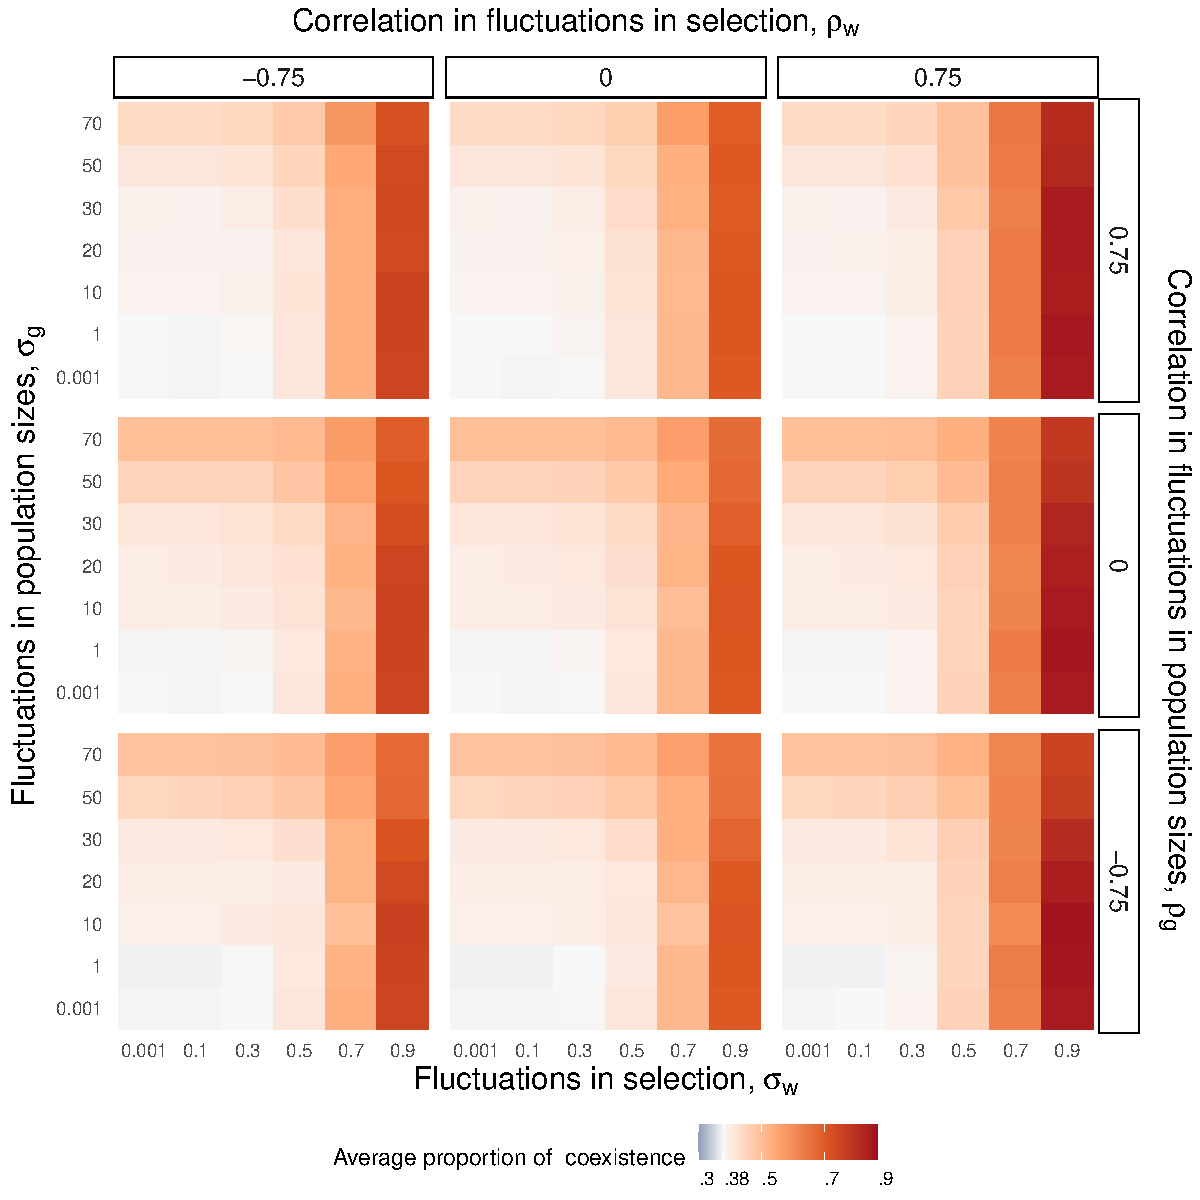
\includegraphics[width=1\textwidth]{heat_map.pdf}}
  \caption{The average proportion of polymorphism maintained in the selection parameter space. For all parameter combinations in our simulations, we show the average proportion of polymorphism in our simulation grids, for all replicates and invasion scenarios (each allele invading a different sex). Each panel corresponds to a different combination of correlations between fluctuations and rows and columns within a pannel show the size of fluctuations in population sizes and in selection, respectively. Labels on top indicate the correlation between fluctuations in selection $\rho_{w}$, while labels on the right show the correlation in fluctuations between fluctuations in population sizes $\rho_{g}$.  As a basis of comparison, we show the expected proportion of polymorphism ($ 0.38$) as white in our color scheme.  }
    \label{fig:heatmap}
\end{figure}


\begin{figure}[H]
  \centerline{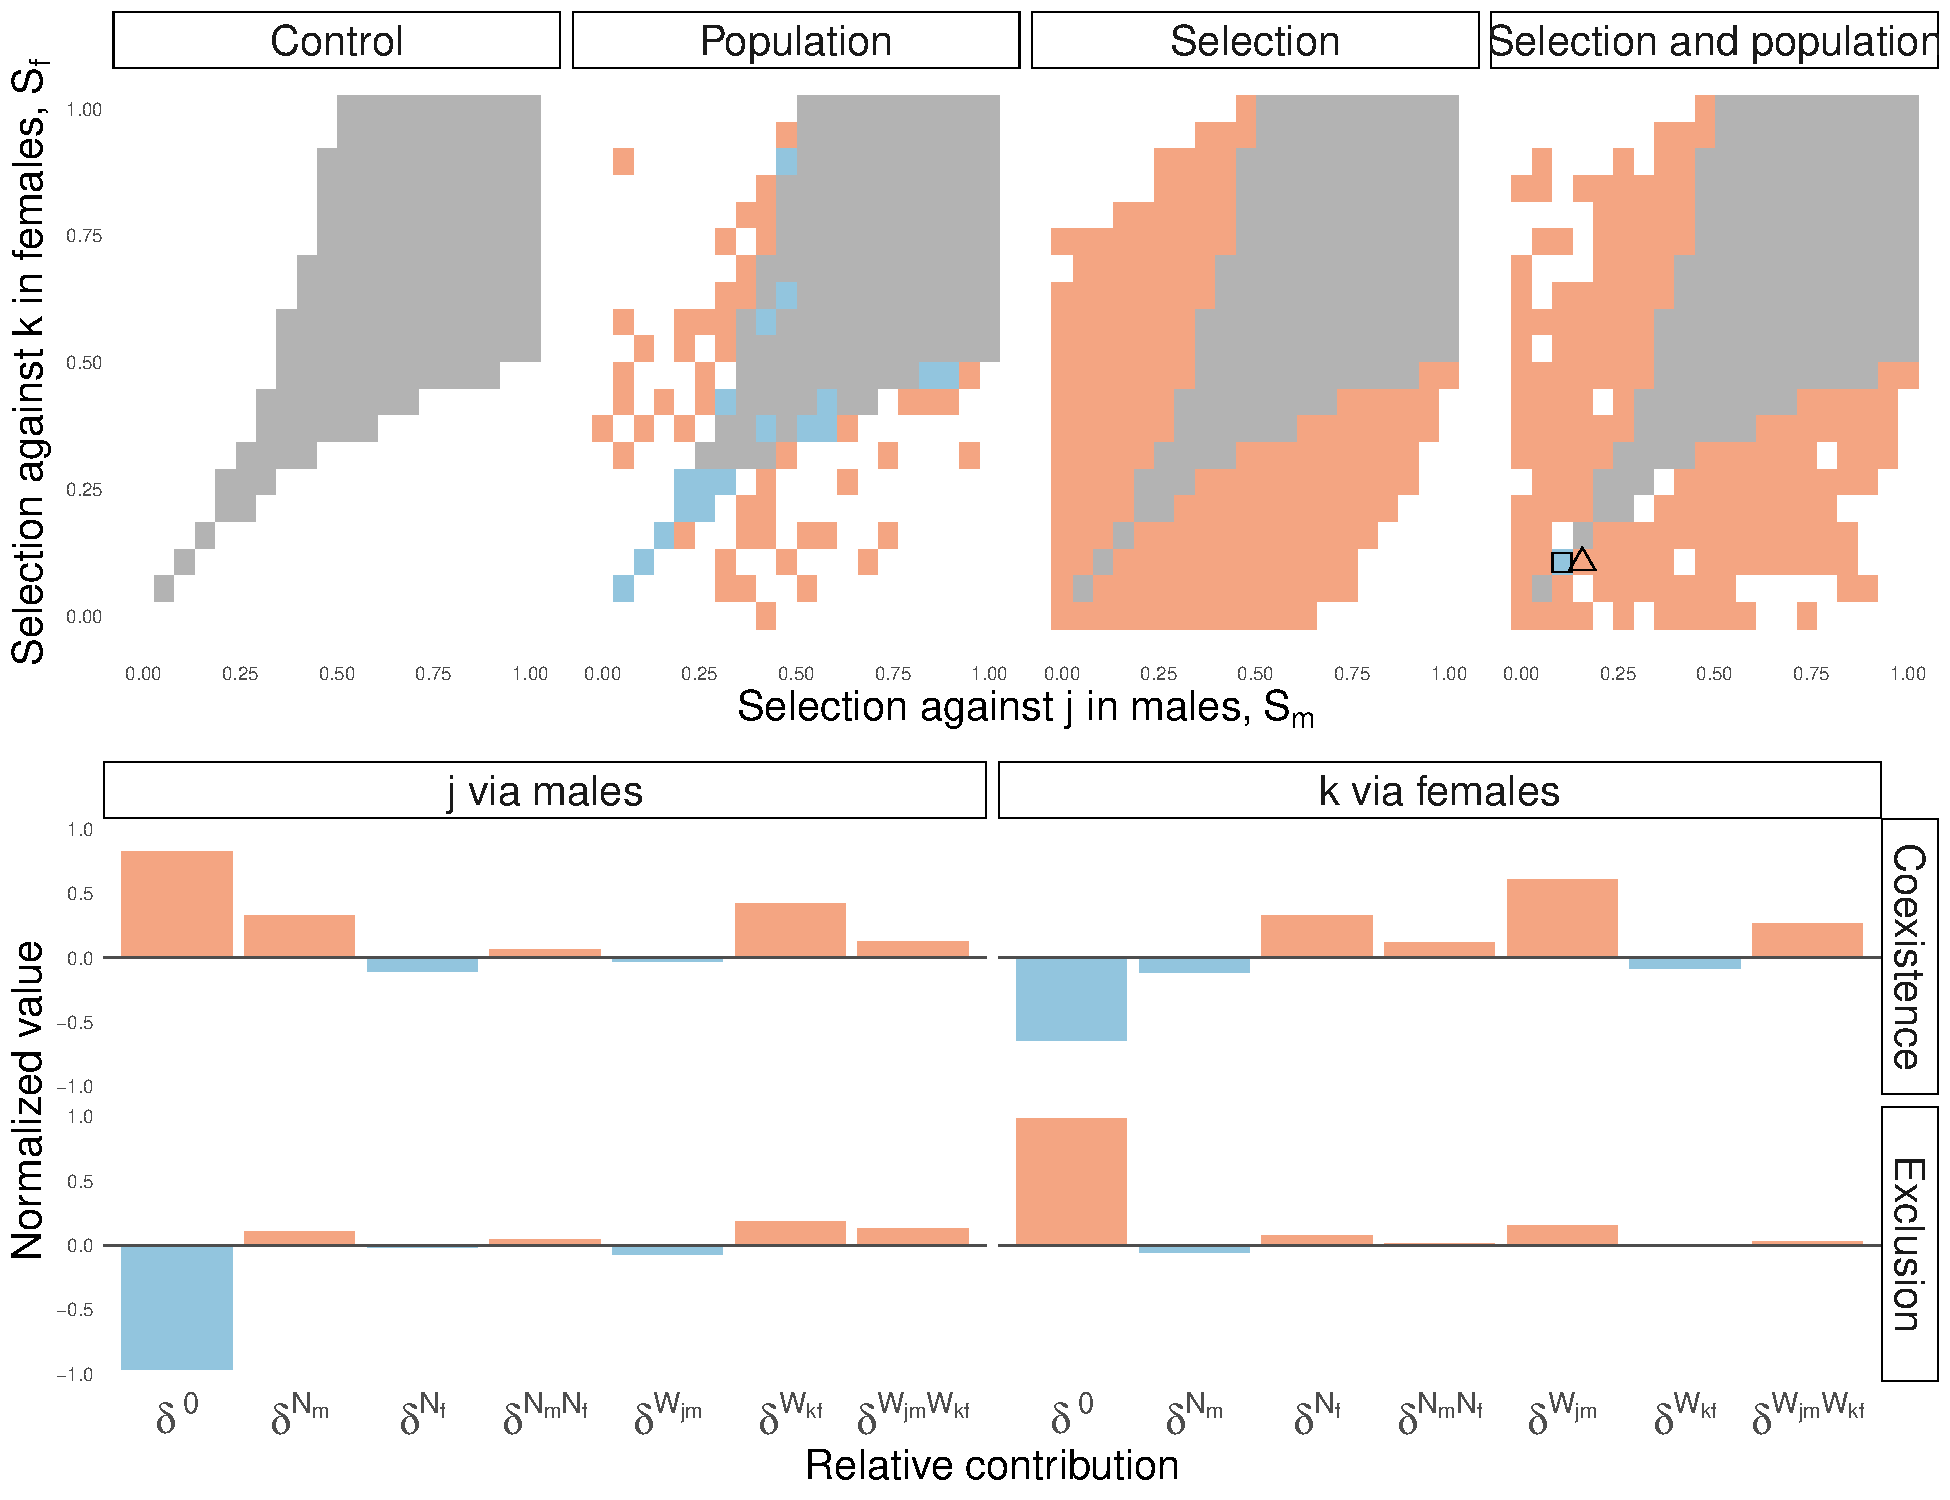
\includegraphics[width=1\textwidth]{outcomes.pdf}}
  \caption{  Maintenance of polymorphism in the parameter space. We show the outcomes of our invasion simulations  when $j$ invaded via males and $k$ invaded via females. As a reference, $j$ is favored in females and $k$ is favored in males. Each panel corresponds to a different replicate of our simulation grids. Grey areas indicate parts of the selection parameter space where polymorphism can be maintained without fluctuations, while white areas indicate parts of the parameter space that correspond to the fixation of one of the alleles (following Eqn.\ref{selection}). Red areas indicate parts of the parameter space where polymorphism can be maintained when fluctuations were incorporated. In A) we show the outcomes of our simulations in the control grid ($\sigma_{g}=0.0001$, $\rho_{g}=0$, $\sigma_{w}=0.0001$, $\rho_{w}=0$). In the B) we show the outcomes when we incorporated high fluctuations in population sizes that were negatively correlated ($\sigma_{g}=70$, $\rho_{g}=-0.75$, $\sigma_{w}=0.001$, $\rho_{w}=0$). In C) we show the outcomes when we incorporated fluctuations in selection that were positively correlated  ($\sigma_{g}=0.0001$, $\rho_{g}=0$, $\sigma_{w}=0.9$, $\rho_{w}=0.75$). Finally, in D) we show the outcomes when both population sizes and selection fluctuated ($\sigma_{g}=70$, $\rho_{g}=-0.75$, $\sigma_{w}=0.9$, $\rho_{w}=0.75$). }
    \label{fig:outcomes}
\end{figure}

%height=1\textheigh

\begin{figure}[H]
  \centerline{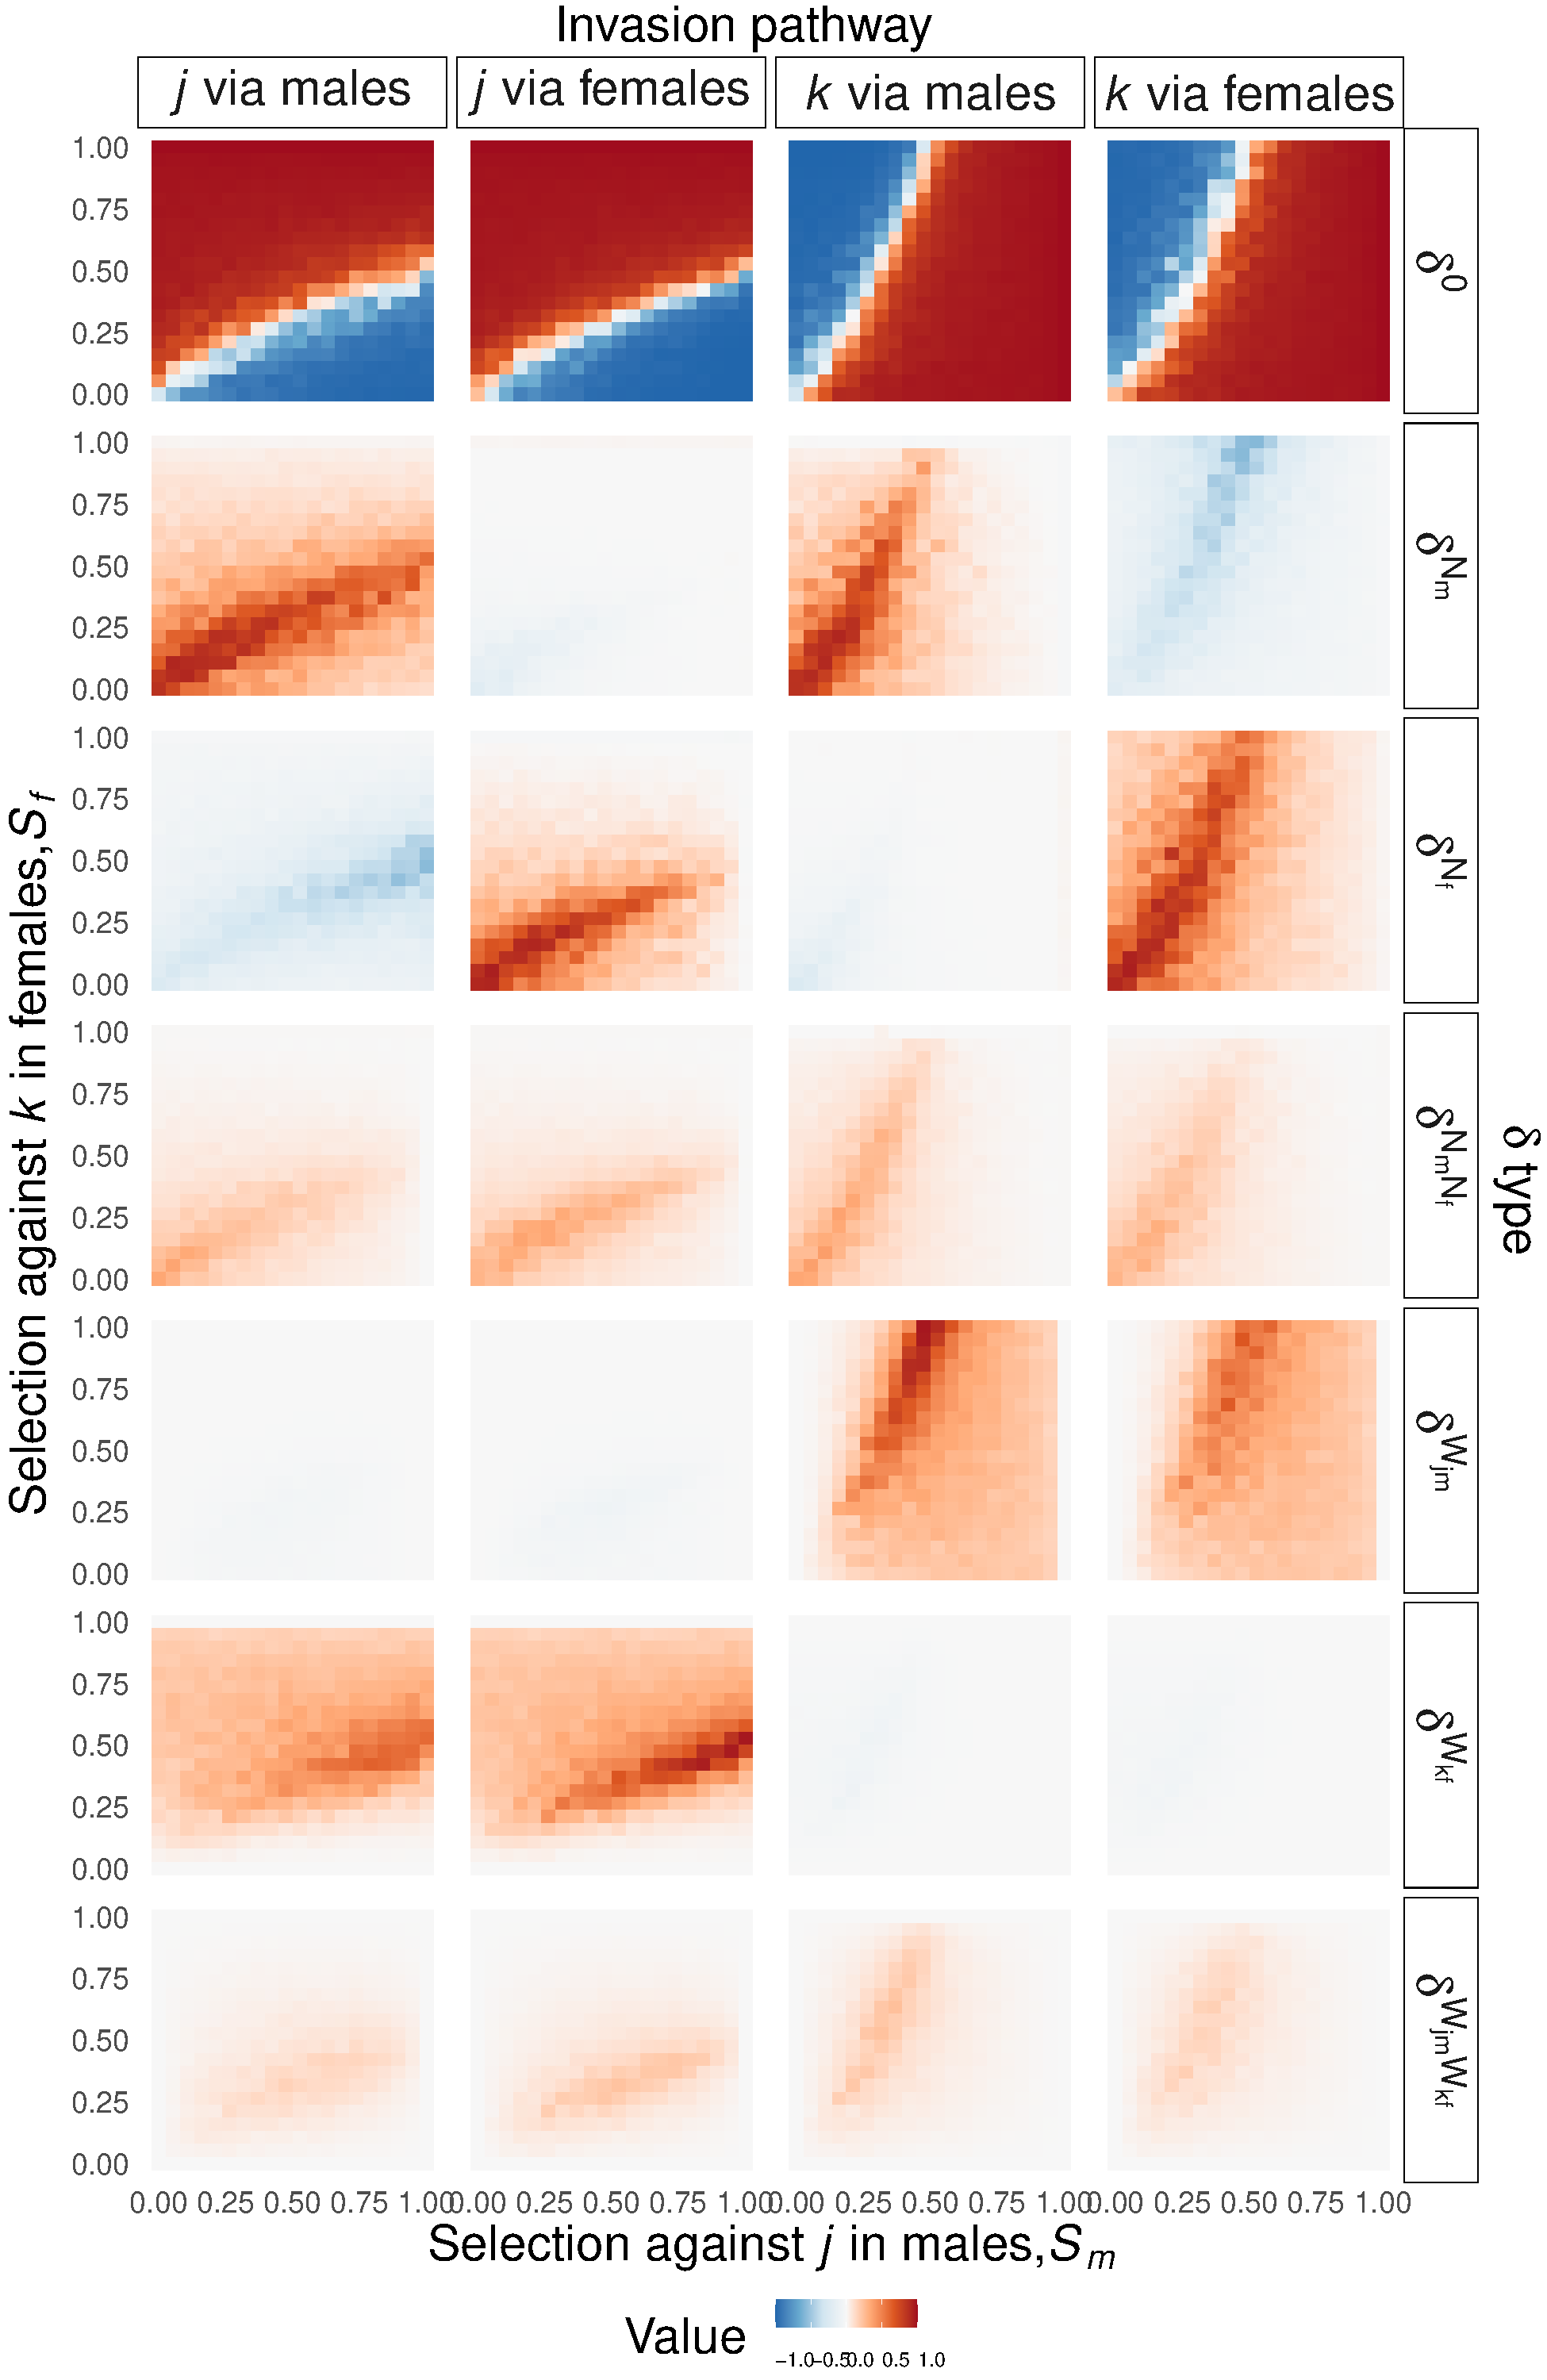
\includegraphics[width=0.9\textwidth]{param_space.pdf}}
    \label{fig:space}
    \captionof{figure}[short caption]{Distribution of $\delta$ values across the parameter space. Caption continued in next page.}
\end{figure}

\addtocounter{figure}{-1}
\begin{figure} [H]
  \caption{ We show the results of the functional decomposition approach for one replicate of our simulation grids where  both population sizes and selection fluctuated with correlated effects  ($\sigma_{g}=70$, $\rho_{g}=-0.75$, $\sigma_{w}=0.9$, $\rho_{w}=0.75$). Each row corresponds to a different type of $\delta$ value, as indicated with labels on the right. Each column corresponds to an allele invading a different pathway, as indicated with labels on top. Areas in red correspond to $\delta$ values that contributed positively to each allele's invasion growth rate, while blue areas denote points in the parameter space where fluctuations had negative contribution to invasion growth rates.  }%missing
    \label{fig:space}
\end{figure}


\begin{figure}[H]
  \centerline{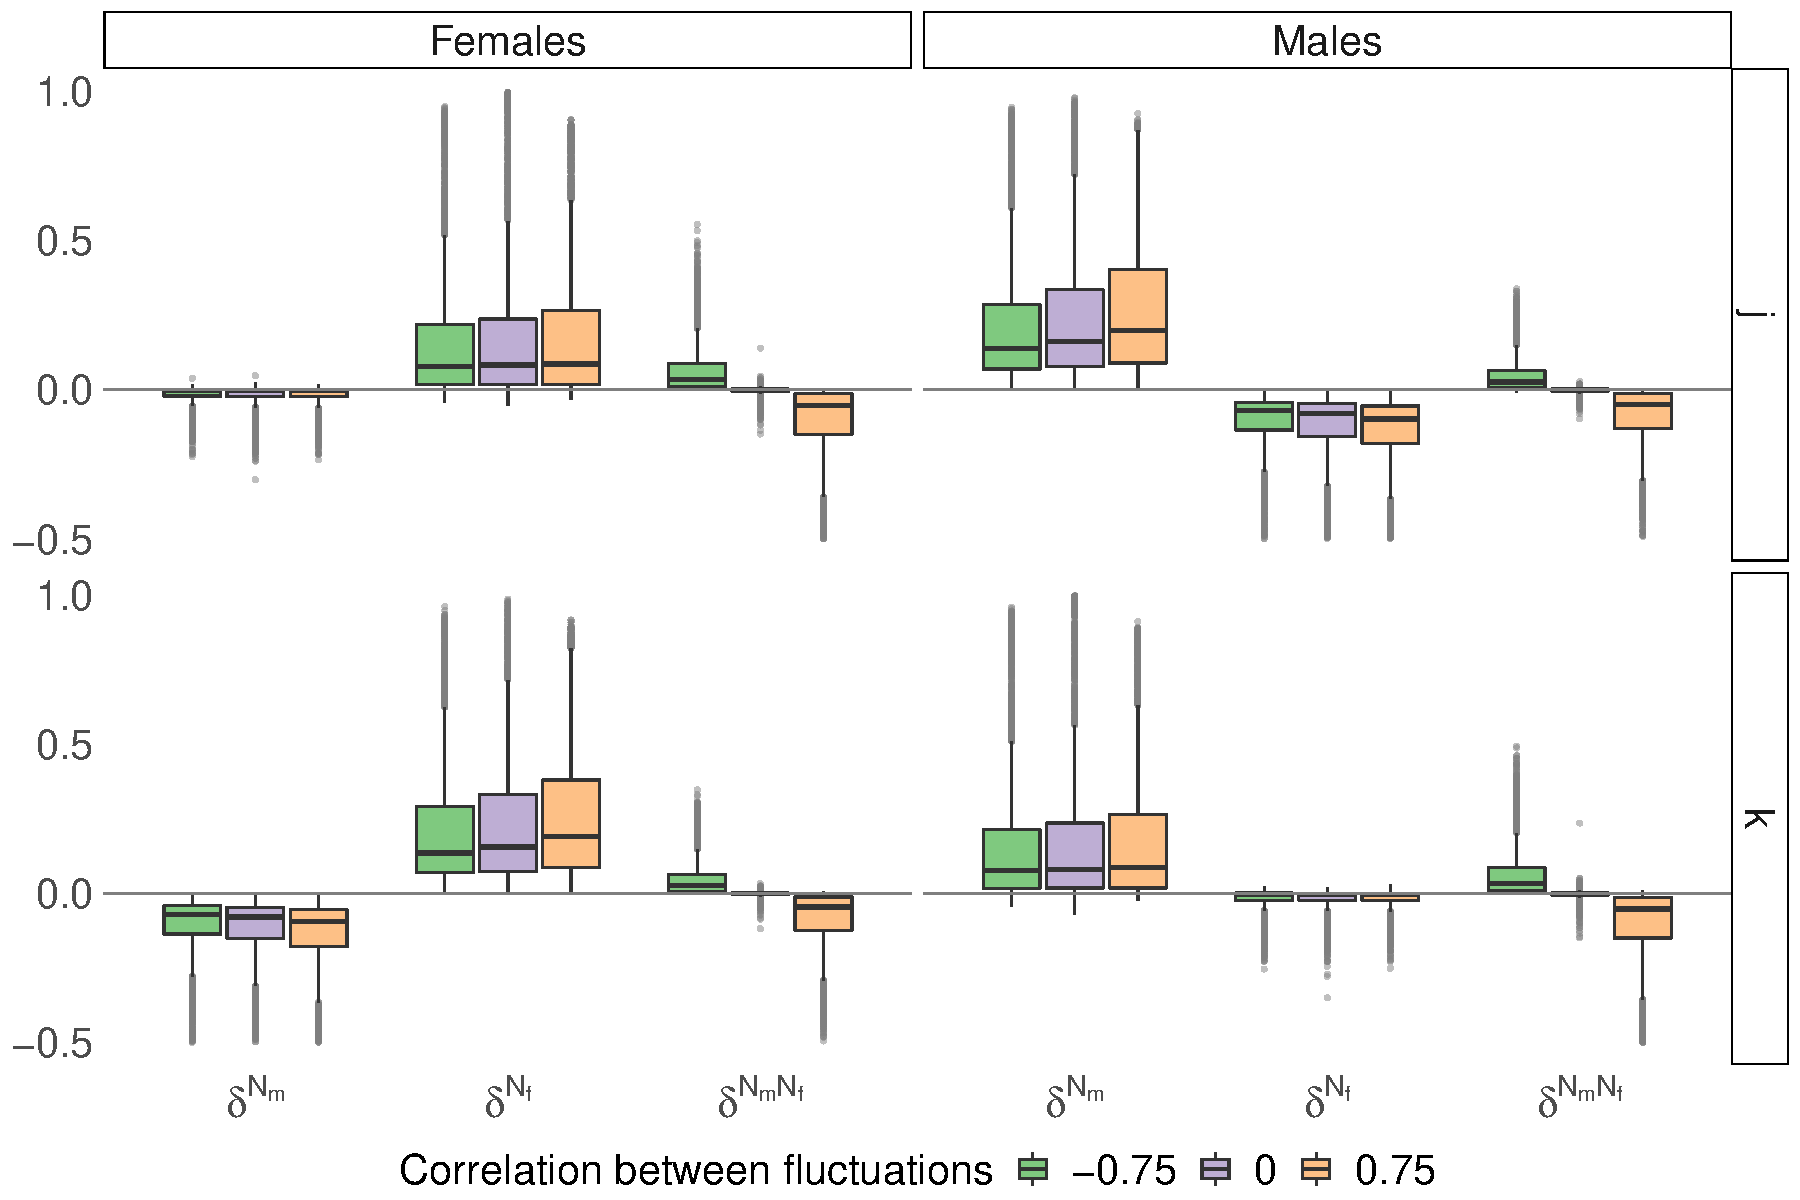
\includegraphics[width=1\textwidth]{box_plots.pdf}}
  \caption{The relative contributions of fluctuations in population sizes to alleles' growth rates when rare. Positive $\delta$ values imply that the corresponding fluctuation benefits that allele as an invader more than the other allele as a resident while negative $\delta$ values indicate fluctuations benefit the residents more than the invader. Each panel corresponds to the result of simulations where each allele invaded via a different pathway, as indicated by top and right labels. We show the boxplots of the three distinct $\delta$ values that captured the effects of fluctuations in population sizes, for all of the replicates in our simulation in which $\sigma_{g}=70$. Each color corresponds to a different correlation between fluctuations in population sizes ($\rho_{g}$), as the legend indicates. Box plots extend from the first to third quantiles of the corresponding $\delta$ values, and the line inside the the box indicates the median. The upper whisker extends to the largest value no further than 1.5 times the inter-quantile range (IQR, or the distance between the first and third quartiles); the lower whisker extends to the smallest value at most 1.5 times the IQR. Data beyond the end of the whiskers are determined to be outliers and are plotted individually with solid grey points. }
    \label{fig:boxes}
\end{figure}



\begin{figure}[H]
  \centerline{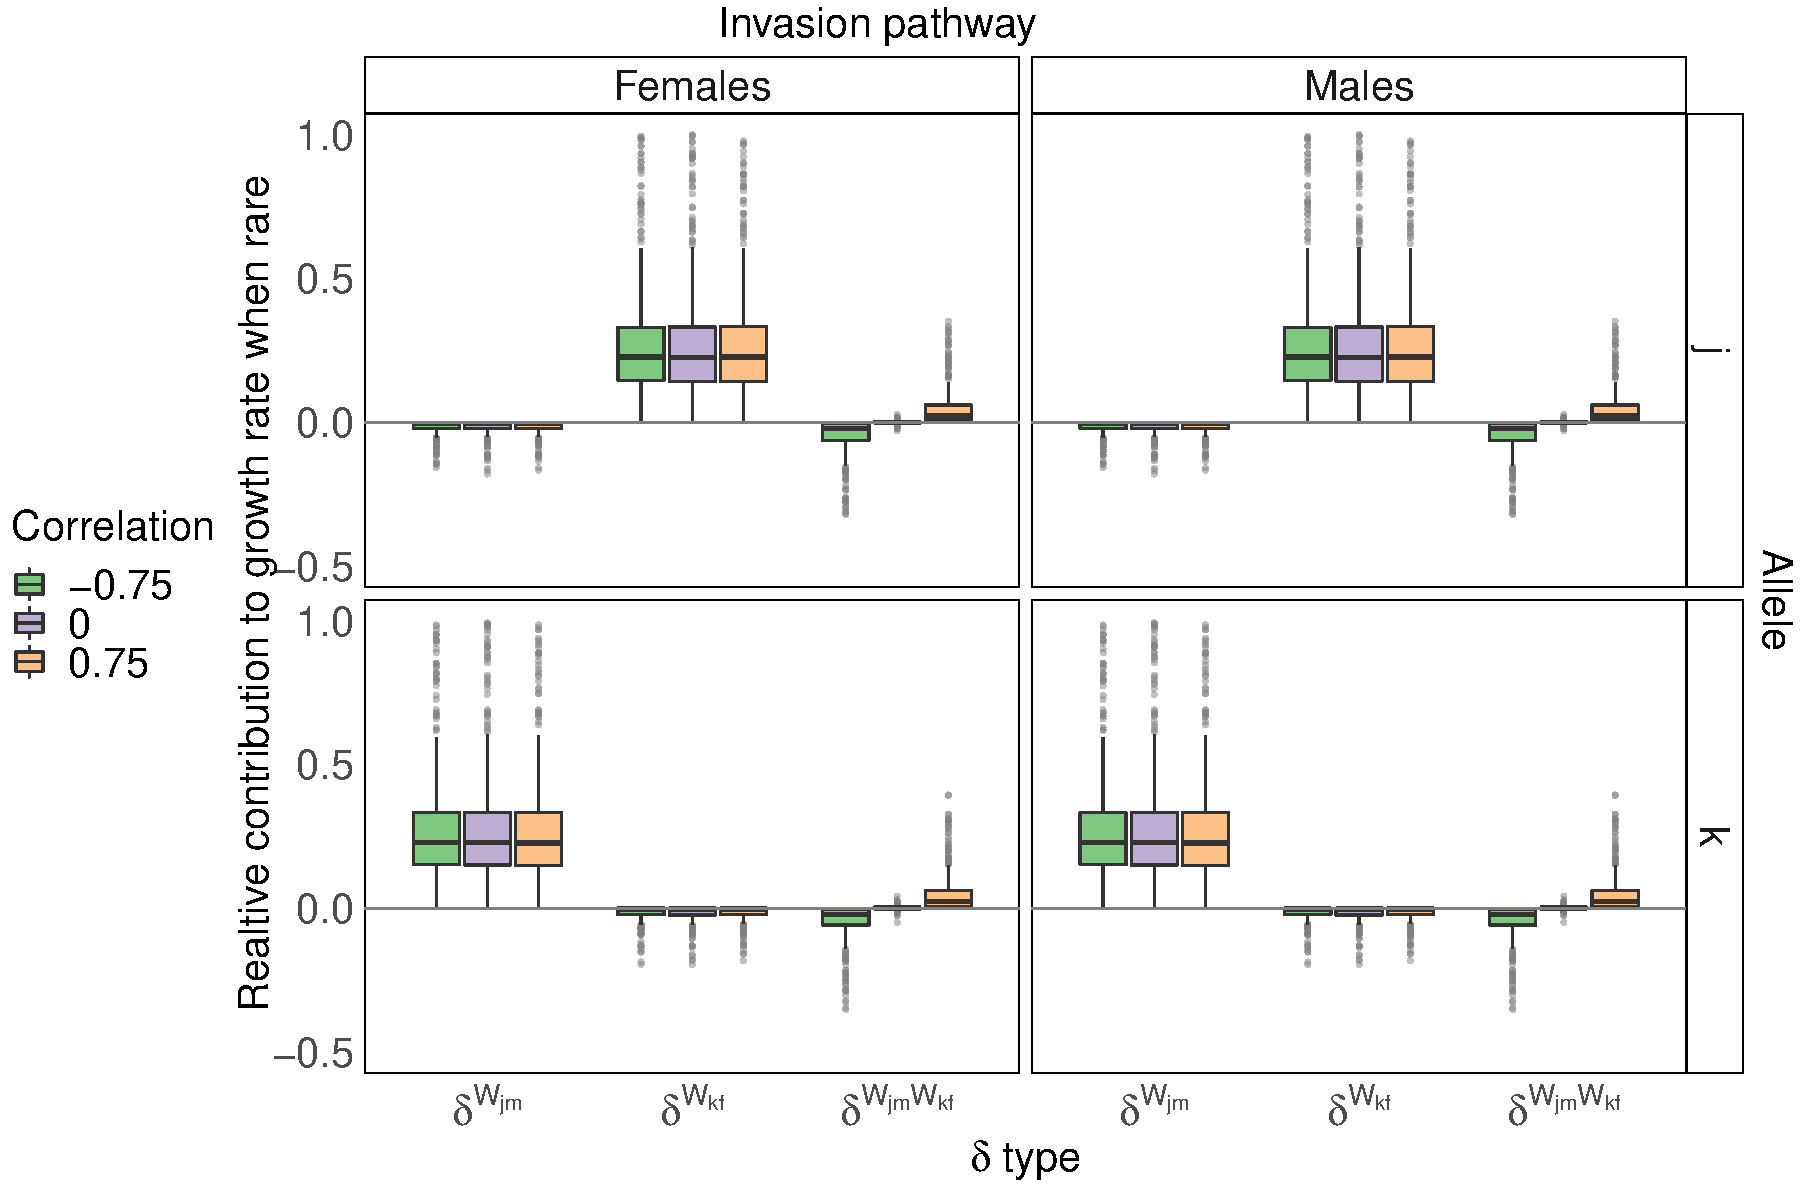
\includegraphics[width=1\textwidth]{box_plots_selection.pdf}}
  \caption{The relative contributions of fluctuations in selection to alleles' growth rates when rare. Positive $\delta$ values imply that the corresponding fluctuation benefits that allele as an invader more than the other allele as a resident while negative $\delta$ values indicate fluctuations benefit the residents more than the invader. Each panel corresponds to the result of simulations where each allele invaded via a different pathway, as indicated by top and right labels. We show the boxplots of the three distinct $\delta$ values that captured the effects of fluctuations in selection, for all of the replicates in our simulation in which $\sigma_{w}=0.9$. Each color corresponds to a different correlation between fluctuations in population sizes ($\rho_{w}$), as the legend indicates. Box plots extend from the first to third quantiles of the corresponding $\delta$ values, and the line inside the the box indicates the median. The upper whisker extends to the largest value no further than 1.5 times the inter-quantile range (IQR, or the distance between the first and third quartiles); the lower whisker extends to the smallest value at most 1.5 times the IQR. Data beyond the end of the whiskers are determined to be outliers and are plotted individually with solid grey points. }
    \label{fig:boxes_selection}
\end{figure}

\clearpage
\bibliographystyle{ecology_letters}
\bibliography{coexistence.bib}

\end{document}
